\documentclass{ethz_report}
\usepackage{listings}
\usepackage{color}
\usepackage{subcaption}

\definecolor{codegreen}{rgb}{0,0.6,0}
\definecolor{codegray}{rgb}{0.5,0.5,0.5}
\definecolor{codepurple}{rgb}{0.58,0,0.82}
\definecolor{backcolour}{rgb}{1,1,1}

\lstdefinestyle{mystyle}{
    backgroundcolor=\color{backcolour},
    commentstyle=\color{codegreen},
    keywordstyle=\color{magenta},
    numberstyle=\tiny\color{codegray},
    stringstyle=\color{codepurple},
    basicstyle=\ttfamily,
    breakatwhitespace=false,
    breaklines=true,
    captionpos=b,
    keepspaces=true,
    numbers=left,
    numbersep=5pt,
    showspaces=false,
    showstringspaces=false,
    showtabs=false,
    tabsize=4,
    frame=lines
}
\lstset{style=mystyle}

\title{Assignment 2 - Locality Sensitive Hashing}
\subject{Data Mining: Learning from Large Datasets}
\author{Alberto Montes}
\email{malberto@student.ethz.ch}
\date{\today}

\begin{document}
\maketitle

\section*{Problem 1: LSH for the Cosine Distance}

The purpose of the following exercise is to simulate and demonstrate that the following family of hash functions:

\begin{equation}
    \mathcal{H} = \{ h(\mathbf{v}) = sign(\mathbf{w}^T \mathbf{v}) \text{ for some } \mathbf{w} \in \mathbb{R}^d \text{ s.t. } ||\mathbf{w}||_2 = 1 \}
\end{equation}

present a probability of collision which depends on the angle as follows:

\begin{equation}
    Pr([h(\mathbf{u})=h(\mathbf{v})]) = 1 - angle(\mathbf{u}, \mathbf{v}) / \pi
    \label{eq:similarity}
\end{equation}

\subsection*{Demonstration}

Lets consider the plane formed by the vectors $\mathbf{u}$ and $\mathbf{v}$. In addition, $\mathbf{w}^T\mathbf{v} = \mathbf{\tilde{w}}^T\mathbf{v}$ being $\mathbf{\tilde{w}}$ the projection of $\mathbf{w}$ that lies to the plane defined by $\mathbf{u}$ and $\mathbf{v}$. With this definition, it can be also considered that the distribution of the angle formed by any of the vectors it is uniformly distributed.

With this definition, we can take into account that:

\begin{equation}
    \mathbf{w}^T\mathbf{u} > 0 \text{ iif } angle(\mathbf{w}) > angle(\mathbf{u})
\end{equation}

With this property, it can be easily deduced that the hash function will give a collision if the random vector $\mathbf{w}$ has an angle larger than the angle of the two vectors $\mathbf{u}$ and $\mathbf{v}$ or if the angle is lower than both of them. (Lets consider that the $angle(\mathbf{u}) > angle(\mathbf{v})$)

\begin{equation}
    sign(\mathbf{w}^T\mathbf{u}) = sign(\mathbf{w}^T\mathbf{u}) = 1 \text{ iif } angle(\mathbf{w}) > angle(\mathbf{u}) > angle(\mathbf{v}) \\
\end{equation}
\begin{equation}
    sign(\mathbf{w}^T\mathbf{u}) = sign(\mathbf{w}^T\mathbf{u}) = -1 \text{ iif } angle(\mathbf{u}) > angle(\mathbf{v}) > angle(\mathbf{w})
\end{equation}

So the probability of collision will depend on the region where the vector $\mathbf{\tilde{w}}$ lies and the relation between its angle and the angle of $\mathbf{u}$ and $\mathbf{v}$.
The probability of collision will be the complementary to the probability of $\mathbf{\tilde{w}}$ to lie between the $\mathbf{u}$ and $\mathbf{v}$ vectors.

\begin{equation}
    P[h_w(\mathbf{u}) = h_w(\mathbf{v})] = 1 - P(angle(\mathbf{u}) > angle(\mathbf{w}), angle(\mathbf{w}) > angle(\mathbf{v}))
\end{equation}

As the distribution of the angles are uniformly distributed, the probability of collision can be easily deduced.

\begin{equation}
    P[h_w(\mathbf{u}) = h_w(\mathbf{v})] = 1 - angle(\mathbf{u}, \mathbf{v}) / \pi
\end{equation}

\subsection*{Implementation}

To simulate this it has been decided to run the simulation with a large number of pairs, in our case: $N = 10^4$. It has also been decided to use 1000 hash functions to get a good precission on the probability of collision for the presented hash function family, so $M = 1000$.

As specified at the statement, all the vectors could initialized as uniformly from $\{-1,+1\}^d$ or normally distributed. For all the simulation, the vectors have been initialized uniformly and for the first simulations, the dimension of the vectors have been set to 10 (so $d=10$). Here is a snippet of how all the vectors are initialized and the angle computed:

\lstinputlisting[language=Python, caption=How the vectors are initialized and the angle computed, firstline=1, lastline=14]{../code/simulation.py}

In addition, it has been implemented the hash function as follows:

\lstinputlisting[language=Python, caption=Hash function implementation, firstline=15, lastline=19]{../code/simulation.py}

For the simulation, if has been generated $N$ pairs of $d$ dimensional vectors, and for each pair, it has been computed the \texttt{hash\_H} for each one of the $M$ hash functions and then compute the probability of collision. For each pair of vectors, also, it has been computed its angle and then plot both variables in an scatter plot.

On the following snippet there is the code that runs the simulation:

\lstinputlisting[language=Python, caption=Simulation code, firstline=21, lastline=50]{../code/simulation.py}

\subsection*{Results}

With the previous implementation and the values set to: $N = 10^4$, $M = 1000$ and $d = 10$,
it has been plot the $Pr([h(\mathbf{u})=h(\mathbf{v})])$ against the $angle(\mathbf{u}, \mathbf{v})$ (Figure~\ref{fig:angle_10}) and $1 - angle(\mathbf{u}, \mathbf{v}) / \pi$ (Figur~\ref{fig:similarity_10}).

\begin{figure}[h]
\centering
\begin{subfigure}[b]{.5\textwidth}
    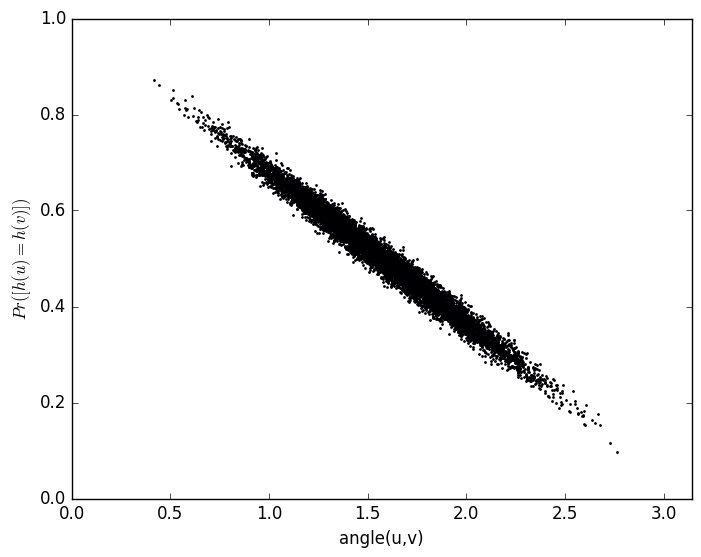
\includegraphics[width=1\linewidth]{../code/simulation_vs_angle_10.png}
    \caption{Probability of collision against angle}
    \label{fig:angle_10}
\end{subfigure}%
\begin{subfigure}[b]{.5\textwidth}
    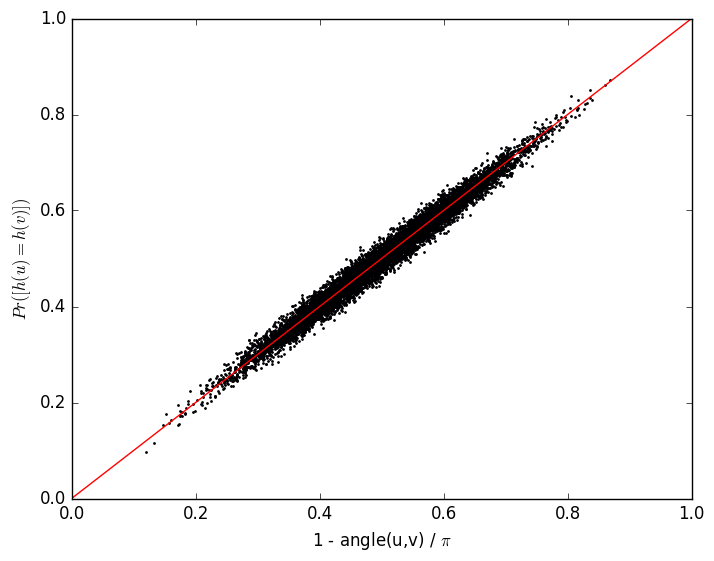
\includegraphics[width=1\linewidth]{../code/simulation_vs_similarity_10.png}
    \caption{Probability of collision agains angular similarity}
    \label{fig:similarity_10}
\end{subfigure}
\caption{Scatter plot of simulation with $d=10$}
\label{fig:d_10}
\end{figure}

On Figure~\ref{fig:d_10} it can be observed how there is a linear correlation between the angle between each pair of vectors and the probability of collision of the hash function family.
In Figure~\ref{fig:similarity_10} can be observed how the correlation is the identity and prove the Equation~\ref{eq:similarity}.

The next simulations where performed changing the dimension of the vectors an testing with the following values of $d = \{2, 5, 10, 20, 50, 100\}$. At Figure~\ref{fig:comparison_d} there is the results.

On this results, it can be observed how at higher dimensions, with a uniform initialization of the vectors, the angle between pairs become more concentrated and so the probability of collision. On the other hand in low dimensions, the angle between pairs and the probability of collision of the hash functions are wider, but this reduce the possible hashes.

\begin{figure}[h]
\centering
\begin{subfigure}[b]{.5\textwidth}
    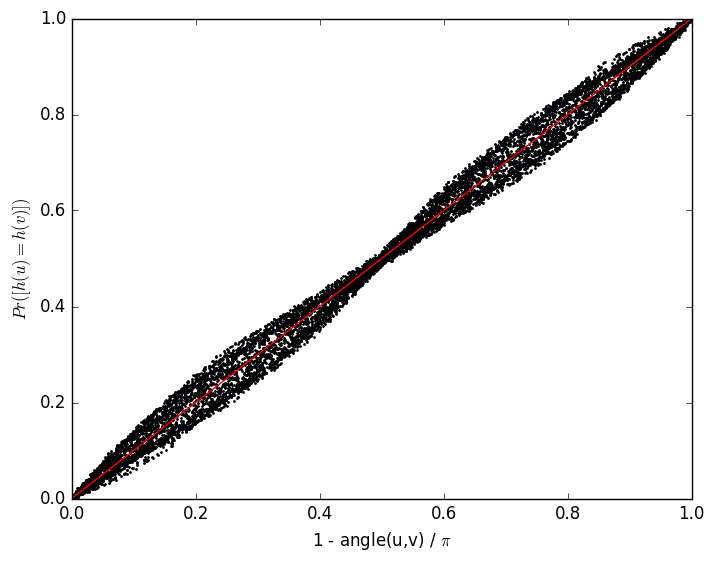
\includegraphics[width=1\linewidth]{../code/simulation_vs_similarity_2.png}
    \caption{$d = 2$}
\end{subfigure}%
\begin{subfigure}[b]{.5\textwidth}
    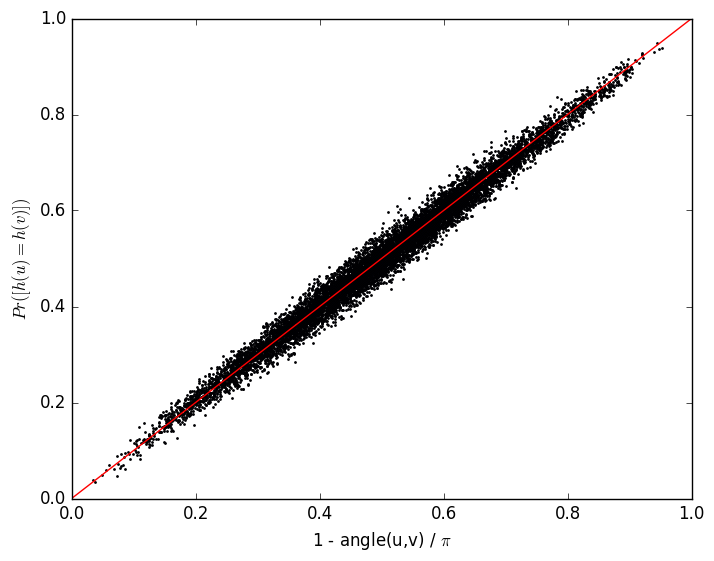
\includegraphics[width=1\linewidth]{../code/simulation_vs_similarity_5.png}
    \caption{$d = 5$}
\end{subfigure}
\begin{subfigure}[b]{.5\textwidth}
    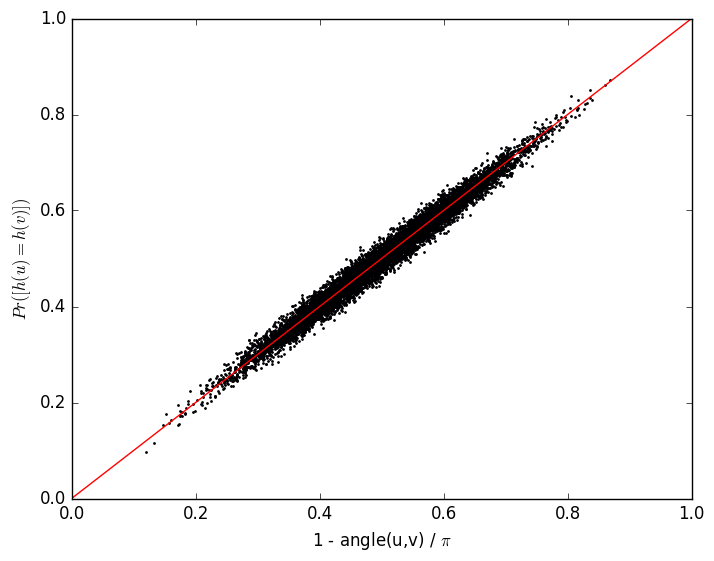
\includegraphics[width=1\linewidth]{../code/simulation_vs_similarity_10.png}
    \caption{$d = 10$}
\end{subfigure}%
\begin{subfigure}[b]{.5\textwidth}
    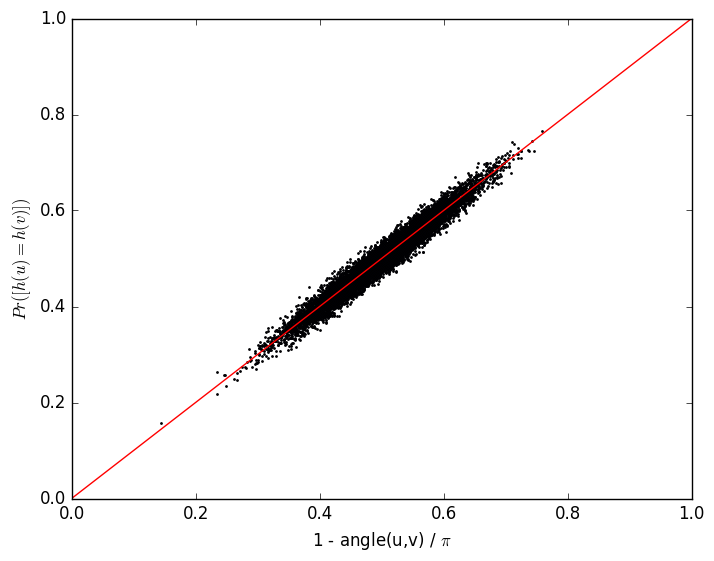
\includegraphics[width=1\linewidth]{../code/simulation_vs_similarity_20.png}
    \caption{$d = 20$}
\end{subfigure}
\begin{subfigure}[b]{.5\textwidth}
    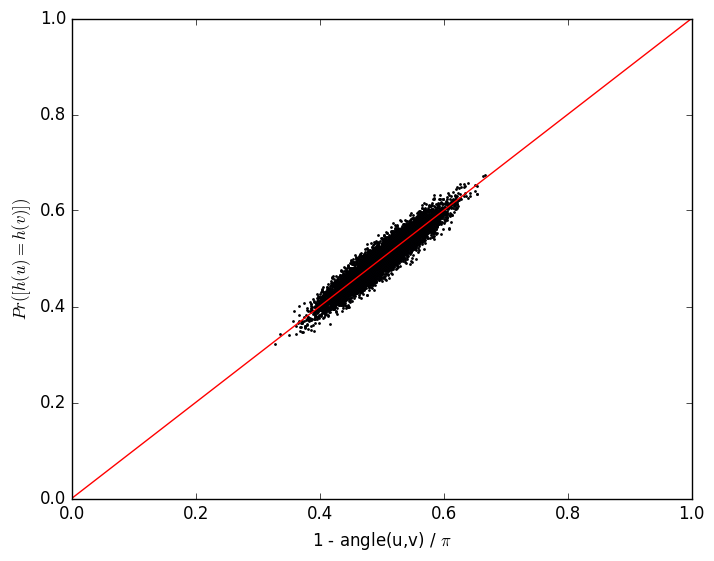
\includegraphics[width=1\linewidth]{../code/simulation_vs_similarity_50.png}
    \caption{$d = 50$}
\end{subfigure}%
\begin{subfigure}[b]{.5\textwidth}
    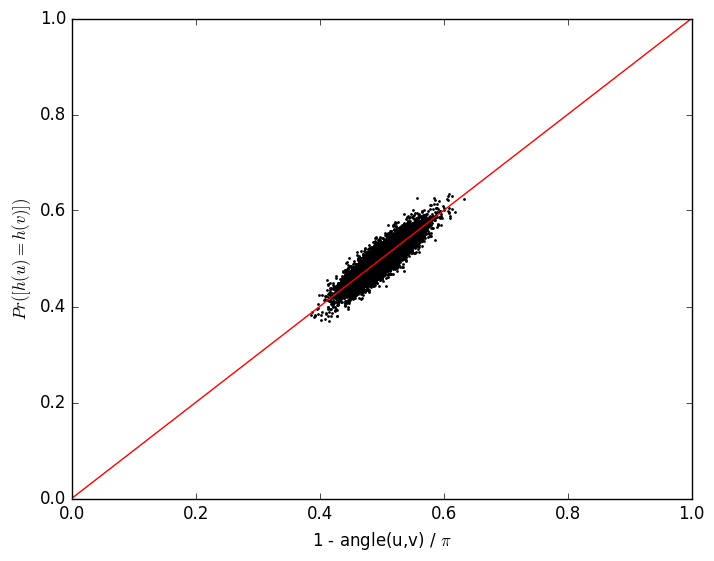
\includegraphics[width=1\linewidth]{../code/simulation_vs_similarity_100.png}
    \caption{$d = 100$}
\end{subfigure}
\caption{Comparison for different values of $d$.}
\label{fig:comparison_d}
\end{figure}


\end{document}
